%%% template.tex
%%%
%%% This LaTeX source document can be used as the basis for your technical
%%% paper or abstract. Intentionally stripped of annotation, the parameters
%%% and commands should be adjusted for your particular paper - title,
%%% author, article DOI, etc.
%%% The accompanying ``template.annotated.tex'' provides copious annotation
%%% for the commands and parameters found in the source document. (The code
%%% is identical in ``template.tex'' and ``template.annotated.tex.'')

\documentclass[conference]{acmsiggraph}

\TOGonlineid{45678}
\TOGvolume{0}
\TOGnumber{0}
\TOGarticleDOI{1111111.2222222}
\TOGprojectURL{}
\TOGvideoURL{}
\TOGdataURL{}
\TOGcodeURL{}

\title{Painterly Rendering for WebGL}

\author{Andy Hanson\thanks{email: hansoa2@rpi.edu}\\
        Scott Todd\thanks{email: todds@rpi.edu}}
\pdfauthor{Robert A. Smith}

\keywords{radiosity, global illumination, constant time}

\begin{document}

\teaser{
  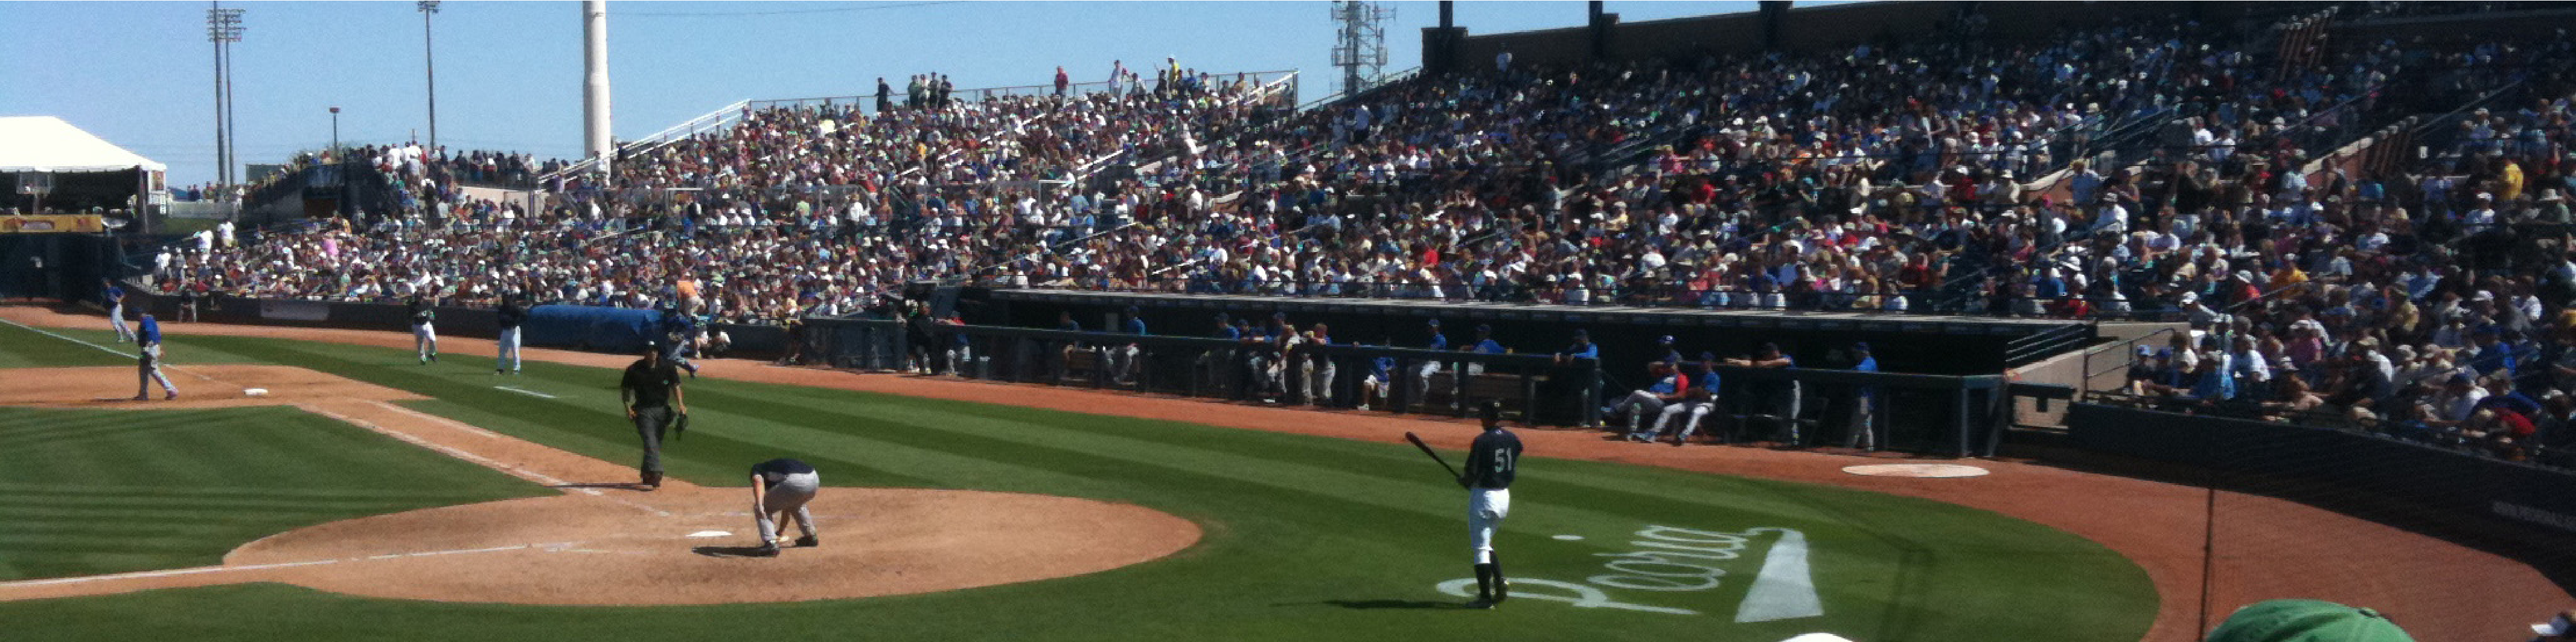
\includegraphics[height=1.5in]{images/sampleteaser}
  \caption{Spring Training 2009, Peoria, AZ.}
}

\maketitle

\begin{abstract}

TODO.

\end{abstract}

%%% The ``CRCatlist'' environment defines one or more ACM ``Computing Review''
%%% (or ``CR'') categories, used for indexing your work. For more information
%%% on CR categories, please see http://www.acm.org/class/1998.

% \begin{CRcatlist}
%   \CRcat{I.3.3}{Computer Graphics}{Three-Dimensional Graphics and Realism}{Display Algorithms}
%   \CRcat{I.3.7}{Computer Graphics}{Three-Dimensional Graphics and Realism}{Radiosity};
% \end{CRcatlist}

\keywordlist

%% Use this only if you're preparing a technical paper to be published in the
%% ACM 'Transactions on Graphics' journal.

\TOGlinkslist

%% Required for all content.

\copyrightspace

\section{Introduction}

TODO.

(Link to GitHub and hosted url)

\subsection{Related Work}

TODO \cite{Meier:1996:PRA:237170.237288}.

\section{Painterly Rendering System}

\subsection{Algorithm Overview}

Our system takes as input a set of three.js geometries and a list of rendering
parameters for each geometry, as well as a list of three.js directional lights.
It outputs to a three.js WebGL renderer in any supporting browser.

TODO.

\begin{figure}[ht]
  \centering
  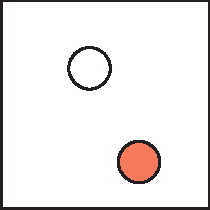
\includegraphics[width=1.5in]{images/samplefigure}
  \caption{Sample illustration.}
\end{figure}

\subsection{Stroke Selection}

TODO.

\section{Stroke Rendering}

\subsection{zQuality}

TODO.

\subsection{Gradient Estimation}

TODO.

\subsection{Layering}

TODO.

\subsection{Parameters List}

TODO.

\section{Results}

TODO.

\section{Limitations}

TODO.

\section{Future Work}

TODO.

\section{Conclusion}

TODO.

\section*{Acknowledgements}

(TODO) Three.js

\bibliographystyle{acmsiggraph}
\bibliography{painterly_rendering}
\end{document}
